% Model report generated by SolverMapp.
% Compile with pdflatex (twice, for the equation and algorithm references).
\documentclass[11pt,a4paper]{article}
\usepackage[T1]{fontenc}
\usepackage[utf8]{inputenc}
\usepackage{lmodern}
\usepackage{amsmath,amssymb}
\usepackage{booktabs,longtable}
\usepackage{siunitx}
\usepackage{algorithm}
\usepackage{algpseudocode}
\usepackage{tikz}
\usetikzlibrary{positioning,shapes.geometric,shapes.misc,arrows.meta}
\usepackage{adjustbox}
\usepackage[hidelinks]{hyperref}

\title{ODE systems: cooling with a heat-flux equation, forced oscillator}
\author{}
\date{\today}

\begin{document}
\maketitle

The model consists of 6 equations in 14 variables: 8 inputs, 3 state variables, 2 intermediate variables and 1 output. It is solved in 3 steps (Algorithm~\ref{alg:solution}).

\section{Nomenclature}
\begin{longtable}{@{}l p{0.48\linewidth} l l@{}}
  \toprule
  Symbol & Description & Unit & Value \\
  \midrule
  \endhead
  \bottomrule
  \endfoot
  \multicolumn{4}{@{}l}{\textit{Inputs}} \\
  $h$ & Heat transfer coefficient & \si{W/(m^{2}.K)} & \num{10} \\
  $A$ & Area & \si{m^{2}} & \num{0.01} \\
  $T_\infty$ & Ambient & \si{K} & \num{293} \\
  $m$ & Mass & \si{kg} & \num{0.1} \\
  $c_p$ & Heat capacity & \si{J/(kg.K)} & \num{900} \\
  $t$ & Time & \si{s} & \num{0} \\
  $F_0$ & Forcing amplitude & \si{m/s^{2}} & \num{0.5} \\
  $\omega$ & Angular frequency & \si{1/s} & \num{2} \\
  \addlinespace
  \multicolumn{4}{@{}l}{\textit{State variables}} \\
  $T$ & Temperature & \si{K} & \num{373} \\
  $v$ & Velocity & \si{m/s} & \num{0} \\
  $x$ & Position & \si{m} & \num{1} \\
  \addlinespace
  \multicolumn{4}{@{}l}{\textit{Intermediate variables}} \\
  $\dot{Q}$ & Heat flux & \si{W} &  \\
  $F$ & Forcing & \si{m/s^{2}} &  \\
  \addlinespace
  \multicolumn{4}{@{}l}{\textit{Outputs}} \\
  $E_k$ & Energy & \si{m^{2}/s^{2}} &  \\
\end{longtable}

\section{Governing equations}

\subsection{Heat flux}
\begin{equation}
  \dot{Q} = h A (T - T_\infty)
  \label{eq:heat-flux}
\end{equation}
\noindent where

\noindent\begin{tabular}{@{\quad}l@{\quad}p{0.7\linewidth}@{}}
  $\dot{Q}$ & Heat flux, \si{W} \\
  $h$ & Heat transfer coefficient, \si{W/(m^{2}.K)} \\
  $A$ & Area, \si{m^{2}} \\
  $T$ & Temperature, \si{K} \\
  $T_\infty$ & Ambient, \si{K} \\
\end{tabular}


\subsection{Cooling}
\begin{equation}
  \frac{dT}{dt} = -\frac{\dot{Q}}{m c_p}
  \label{eq:cooling}
\end{equation}
\noindent where

\noindent\begin{tabular}{@{\quad}l@{\quad}p{0.7\linewidth}@{}}
  $T$ & Temperature, \si{K} \\
  $\dot{Q}$ & Heat flux, \si{W} \\
  $m$ & Mass, \si{kg} \\
  $c_p$ & Heat capacity, \si{J/(kg.K)} \\
  $t$ & Time, \si{s} \\
\end{tabular}

\noindent Integrated over $t$ from $0$ to $600$ with the classical fourth-order Runge–Kutta method in 60 steps, starting from the start value of $T$.

\subsection{Forcing}
\begin{equation}
  F = F_0 \sin(\omega t)
  \label{eq:forcing}
\end{equation}
\noindent where

\noindent\begin{tabular}{@{\quad}l@{\quad}p{0.7\linewidth}@{}}
  $F$ & Forcing, \si{m/s^{2}} \\
  $F_0$ & Forcing amplitude, \si{m/s^{2}} \\
  $\omega$ & Angular frequency, \si{1/s} \\
  $t$ & Time, \si{s} \\
\end{tabular}


\subsection{Position}
\begin{equation}
  \frac{dx}{dt} = v
  \label{eq:position}
\end{equation}
\noindent where

\noindent\begin{tabular}{@{\quad}l@{\quad}p{0.7\linewidth}@{}}
  $x$ & Position, \si{m} \\
  $v$ & Velocity, \si{m/s} \\
  $t$ & Time, \si{s} \\
\end{tabular}

\noindent Integrated over $t$ from $0$ to $3$ with the classical fourth-order Runge–Kutta method in 300 steps, starting from the start value of $x$, together with Eq.~\eqref{eq:velocity}.

\subsection{Velocity}
\begin{equation}
  \frac{dv}{dt} = -\omega^2 x + F
  \label{eq:velocity}
\end{equation}
\noindent where

\noindent\begin{tabular}{@{\quad}l@{\quad}p{0.7\linewidth}@{}}
  $v$ & Velocity, \si{m/s} \\
  $\omega$ & Angular frequency, \si{1/s} \\
  $x$ & Position, \si{m} \\
  $F$ & Forcing, \si{m/s^{2}} \\
  $t$ & Time, \si{s} \\
\end{tabular}

\noindent Integrated over $t$ from $0$ to $3$ with the classical fourth-order Runge–Kutta method in 300 steps, starting from the start value of $v$, together with Eq.~\eqref{eq:position}.

\subsection{Energy}
\begin{equation}
  E_k = \frac{1}{2} v^2 + \frac{1}{2} \omega^2 x^2
  \label{eq:energy}
\end{equation}
\noindent where

\noindent\begin{tabular}{@{\quad}l@{\quad}p{0.7\linewidth}@{}}
  $E_k$ & Energy, \si{m^{2}/s^{2}} \\
  $v$ & Velocity, \si{m/s} \\
  $\omega$ & Angular frequency, \si{1/s} \\
  $x$ & Position, \si{m} \\
\end{tabular}


\section{Solution algorithm}
\begin{algorithm}[htbp]
  \caption{Solution procedure}\label{alg:solution}
  \begin{algorithmic}[1]
    \State Set the inputs $h$, $A$, $T_\infty$, $m$, $c_p$, $F_0$ and $\omega$
    \State Set the start values $T$ = \num{373}, $v$ = \num{0} and $x$ = \num{1}
    \For{$t = 0$ to $600$ in 60 steps} \Comment{RK4}
      \State Compute $\dot{Q}$ from Eq.~\eqref{eq:heat-flux}
      \State Advance $T$ by one RK4 step of Eq.~\eqref{eq:cooling} (the equations above are evaluated at each of its 4 stages)
    \EndFor
    \For{$t = 0$ to $3$ in 300 steps} \Comment{RK4}
      \State Compute $F$ from Eq.~\eqref{eq:forcing}
      \State Advance $x$ and $v$ by one RK4 step of Eq.~\eqref{eq:position} and Eq.~\eqref{eq:velocity} (the equations above are evaluated at each of its 4 stages)
    \EndFor
    \State Compute $E_k$ from Eq.~\eqref{eq:energy}
  \end{algorithmic}
\end{algorithm}

Figure~\ref{fig:flowchart} shows the same procedure as a flowchart.

\begin{figure}[htbp]
  \centering
  \begin{adjustbox}{max width=\linewidth, max totalheight=0.9\textheight}
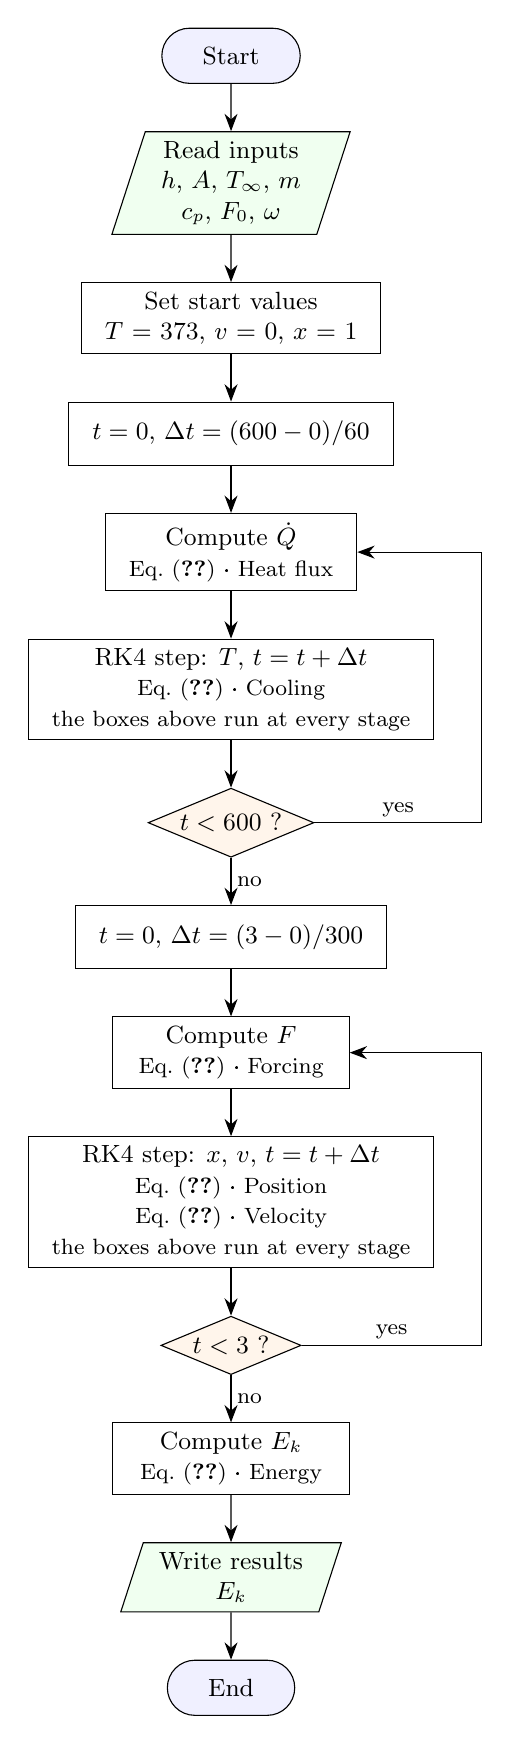
\begin{tikzpicture}[
  node distance=6mm, >={Stealth[length=2.2mm]}, font=\small,
  every node/.style={align=center},
  term/.style={draw, rounded rectangle, minimum height=7mm, inner xsep=5mm, fill=blue!6},
  io/.style={draw, trapezium, trapezium left angle=72, trapezium right angle=108, trapezium stretches body, minimum height=8mm, inner xsep=2mm, fill=green!6},
  proc/.style={draw, rectangle, minimum height=8mm, minimum width=30mm, inner xsep=3mm},
  dec/.style={draw, diamond, aspect=2.4, inner sep=1pt, fill=orange!8},
  lbl/.style={font=\footnotesize, inner sep=2pt}]
  \node[term] (n1) {Start};
  \node[io, below=of n1] (n2) {Read inputs \\ $h$, $A$, $T_\infty$, $m$ \\ $c_p$, $F_0$, $\omega$};
  \node[proc, below=of n2] (n3) {Set start values \\ $T$ = 373, $v$ = 0, $x$ = 1};
  \node[proc, below=of n3] (n4) {$t = 0$, $\Delta t = (600 - 0) / 60$};
  \node[proc, below=of n4] (n5) {Compute $\dot{Q}$ \\ {\footnotesize Eq.~\eqref{eq:heat-flux} \textperiodcentered{} Heat flux}};
  \node[proc, below=of n5] (n6) {RK4 step: $T$, $t = t + \Delta t$ \\ {\footnotesize Eq.~\eqref{eq:cooling} \textperiodcentered{} Cooling} \\ {\footnotesize the boxes above run at every stage}};
  \node[dec, below=of n6] (n7) {$t < 600$ ?};
  \node[proc, below=of n7] (n8) {$t = 0$, $\Delta t = (3 - 0) / 300$};
  \node[proc, below=of n8] (n9) {Compute $F$ \\ {\footnotesize Eq.~\eqref{eq:forcing} \textperiodcentered{} Forcing}};
  \node[proc, below=of n9] (n10) {RK4 step: $x$, $v$, $t = t + \Delta t$ \\ {\footnotesize Eq.~\eqref{eq:position} \textperiodcentered{} Position} \\ {\footnotesize Eq.~\eqref{eq:velocity} \textperiodcentered{} Velocity} \\ {\footnotesize the boxes above run at every stage}};
  \node[dec, below=of n10] (n11) {$t < 3$ ?};
  \node[proc, below=of n11] (n12) {Compute $E_k$ \\ {\footnotesize Eq.~\eqref{eq:energy} \textperiodcentered{} Energy}};
  \node[io, below=of n12] (n13) {Write results \\ $E_k$};
  \node[term, below=of n13] (n14) {End};
  \coordinate (E) at (current bounding box.east);
  \coordinate (L0) at ([xshift=6mm]E);
  \draw[->] (n1) -- (n2);
  \draw[->] (n2) -- (n3);
  \draw[->] (n3) -- (n4);
  \draw[->] (n4) -- (n5);
  \draw[->] (n5) -- (n6);
  \draw[->] (n6) -- (n7);
  \draw[->] (n7) -- node[lbl, right] {no} (n8);
  \draw[->] (n8) -- (n9);
  \draw[->] (n9) -- (n10);
  \draw[->] (n10) -- (n11);
  \draw[->] (n11) -- node[lbl, right] {no} (n12);
  \draw[->] (n12) -- (n13);
  \draw[->] (n13) -- (n14);
  \draw[->] (n7.east) -- node[lbl, above] {yes} (n7.east -| L0) |- (n5.east);
  \draw[->] (n11.east) -- node[lbl, above] {yes} (n11.east -| L0) |- (n9.east);
\end{tikzpicture}
  \end{adjustbox}
  \caption{Flowchart of the solution procedure}\label{fig:flowchart}
\end{figure}

\end{document}